\section{Gegevensmodel}
\subsection{Data format}
Het dataformaat van de u-blox is NMEA, NMEA is een standaardprotocol voor het
weergeven van GPS-data. Dit ziet er zo uit: \\
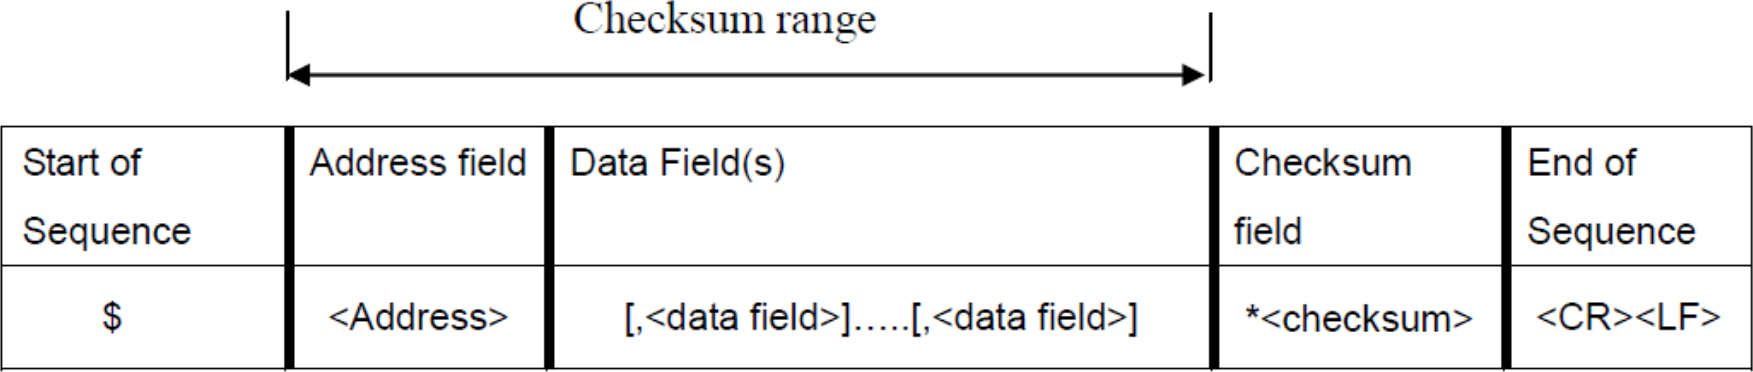
\includegraphics[width=\textwidth]{technical/nmea}
\\Hierbij is het adres veld in het formaat ``aaccc'', waarbij ``aa'' het
Talker ID is en ``ccc'' het soort bericht. Velden zijn gesepareerd met
een ``,''.
\citep{Navspark}\\\\
Het belangrijkste deel van dit format zijn de GNS-berichten
(GNSS-data). Deze berichten zien er als volgt uit:\\
\texttt{\$GPGNS,091547.00,5114.50897,N,00012.28663,W,AA,10,0.83,111.1,45.6,,,V*71}
\\\\
De velden houden in:
\\\\
\begin{tabularx}{\textwidth}{| l | l | l | l | X |}
    \hline
    \textbf{Veld} & \textbf{Naam} & \textbf{Formaat} & \textbf{Voorbeeld} & \textbf{Beschrijving}          \\ \hline
    0             & xxGNS         & string           & \$GPGNS            & GNS ID (xx = current Talker)   \\ \hline
    1             & Tijd          & hhmmss.ss        & 091547.00          & Tijd (UTC)                     \\ \hline
    2             & Latitude      & ddmm.mmmmm       & 5114.50897         & Latitude (graden en minuten)   \\ \hline
    3             & NS            & character        & N                  & Noord/Zuid                     \\ \hline
    4             & Longtitude    & dddmm.mmmmm      & 00012.28663        & Longtitude (graden en minuten) \\ \hline
    5             & EW            & character        & E                  & Oost/West                      \\ \hline
    6             & posMode       & character        & AA                 & Positionering mode             \\ \hline
    7             & numSV         & numeric          & 10                 & Aantal satellieten             \\ \hline
    8             & HDOP          & numeric          & 0.83               & Horizontal dilution precision  \\ \hline
    9             & alt           & numeric          & 111.1              & Hoogte boven zeeniveau         \\ \hline
    10            & sep           & numeric          & 45.6               & Geoïde separatie               \\ \hline
    11            & diffAge       & numeric          & -                  & Leeftijd correctie             \\ \hline
    12            & diffStation   & numeric          & -                  & ID GPS-correctie station       \\ \hline
    13            & navStatus     & character        & V                  & Navigatie Status               \\ \hline
    14            & cs            & hexadecimal      & *71                & Checksum                       \\ \hline
    15            & <CR><LF>      & character        & -                  & Carriage Return                \\ \hline
\end{tabularx}
\citep[p. 116]{UBlox8}\\
Een ander deel van de data die we mogelijk gaan gebruiken is:
\texttt{\$GPGBS}. \texttt{\$GPGBS} bevat de afwijking van de data bij u-blox
DGPS-toestellen.
\citep[p. 111]{UBlox8}

De uiteindelijke data die we gaan gebruiken is:
ID, Tijd (UTC), Latitude, Longtitude en Altitude

Voor het referentiestation komt hier nog bij:
error Latitude, error Longtitude en error Altitude

\subsection{Database}
\label{sec:database}

De Smart Markers versturen hun data naar de KPN LoRa portal.

Vanuit deze portal is het mogelijk om via een https verbinding, welke dus beveiligd is,
te versturen naar een eigen API.

Voor dit project komt het binnen in een PHP script, welke de verkregen data samen met het
moment van ontvangen in een SQL-database zet. Deze database draait op dezelfde server als
de webserver. De meetpunten worden hierbij in de decimale notatie opgeslagen.

Deze server draait bij één van de projectleden thuis. Deze bestaat uit een virtuele
machine met daarop CentOS 7. Deze draait de Apache webserver gecombineerd met een
MariaDB SQL-database.

Het HTTPS certificaat wordt verkregen met een certificaat van Let's Encrypt.org

De tabel met de meetpunten bevat de volgende kolommen:
\begin{itemize}
    \item Meetpunt ID
    \item Marker nummer
    \item Latitude
    \item Longitude
    \item Tijdstip van registratie
\end{itemize}

De tabel percelen bevat de volgende kolommen:
\begin{itemize}
    \item Perceel ID
    \item Perceelnaam
    \item Tijdstip van creëren
\end{itemize}

Om de percelen en meetpunten aan elkaar te koppelen is er een koppeltabel:
\begin{itemize}
    \item Volgnummer
    \item Perceel ID
    \item Meetpunt ID
\end{itemize}

Omdat dit een veel op veel relatie is, een meetpunt kan meerdere percelen begrenzen en
een perceel heeft meerdere meetpunten, is er een koppeltabel nodig. Deze koppelt het id
van een perceel aan het ID van de bijbehorende meetpunten.
